\documentclass[12pt,tikz]{standalone}
\pdfinfoomitdate 1
\pdfsuppressptexinfo 1
\pdftrailerid{}
\usepackage[utf8]{inputenc}
\usepackage{amsmath}
\usepackage{pgfplots}
\usepackage{tikz}
\usetikzlibrary{shapes.geometric}
\pagestyle{empty}

\begin{document}
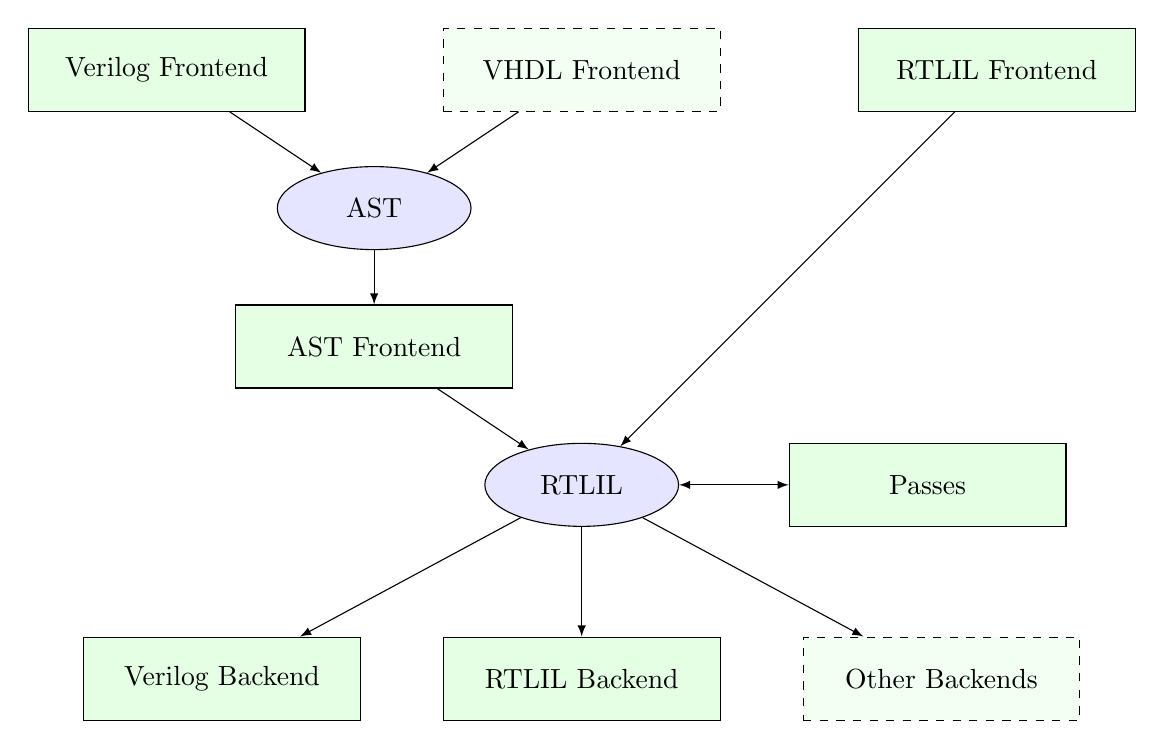
\begin{tikzpicture}
	\tikzstyle{process} = [draw, fill=green!10, rectangle, minimum height=3em, minimum width=10em, node distance=15em]
	\tikzstyle{data} = [draw, fill=blue!10, ellipse, minimum height=3em, minimum width=7em, node distance=15em]
	\node[process] (vlog) {Verilog Frontend};
	\node[process, dashed, fill=green!5] (vhdl) [right of=vlog] {VHDL Frontend};
	\node[process] (ilang) [right of=vhdl] {RTLIL Frontend};
	\node[data] (ast) [below of=vlog, node distance=5em, xshift=7.5em] {AST};
	\node[process] (astfe) [below of=ast, node distance=5em] {AST Frontend};
	\node[data] (rtlil) [below of=astfe, node distance=5em, xshift=7.5em] {RTLIL};
	\node[process] (pass) [right of=rtlil, node distance=5em, xshift=7.5em] {Passes};
	\node[process] (vlbe) [below of=rtlil, node distance=7em, xshift=-13em] {Verilog Backend};
	\node[process] (ilangbe) [below of=rtlil, node distance=7em, xshift=0em] {RTLIL Backend};
	\node[process, dashed, fill=green!5] (otherbe) [below of=rtlil, node distance=7em, xshift=+13em] {Other Backends};

	\draw[-latex] (vlog) -- (ast);
	\draw[-latex] (vhdl) -- (ast);
	\draw[-latex] (ast) -- (astfe);
	\draw[-latex] (astfe) -- (rtlil);
	\draw[-latex] (ilang) -- (rtlil);
	\draw[latex-latex] (rtlil) -- (pass);
	\draw[-latex] (rtlil) -- (vlbe);
	\draw[-latex] (rtlil) -- (ilangbe);
	\draw[-latex] (rtlil) -- (otherbe);
\end{tikzpicture}
\end{document}
